%% GENERATED by tools/from_docs.py from stepss-docs. Do not edit by hand:
%% edit the page named below in stepss-docs and regenerate.
%% source: stepss-docs/src/content/docs/models/injectors/induction-machines.md

\chapter{Induction machine models}\label{doc:model-inj-indmach}

Injector models for induction machines, used as motors or generators.

The \texttt{INJEC} record these models are entered with, and the rules on model names, are on the \hyperref[doc:model-inj]{Injector Models} page.

\section{\texorpdfstring{INDMACH1 (\texttt{inj\_indmach1}): Single-Cage Induction Machine}{INDMACH1 (inj\_indmach1): Single-Cage Induction Machine}}\label{model-inj-indmach:indmach1-inj_indmach1-single-cage-induction-machine}

\subsection{Description}\label{model-inj-indmach:description}

A single-cage (single-rotor-circuit) induction machine model for motor loads. The machine is represented on its own MVA base (or inferred from load factor \texttt{LF}) with a shunt capacitor \(B_{\mathrm{sh}}\) to represent power factor correction. The mechanical torque is a quadratic function of rotor speed. At initialization, the model solves nonlinear algebraic equations to find the operating-point slip and flux linkages.

\begin{figure}[htbp]
\centering
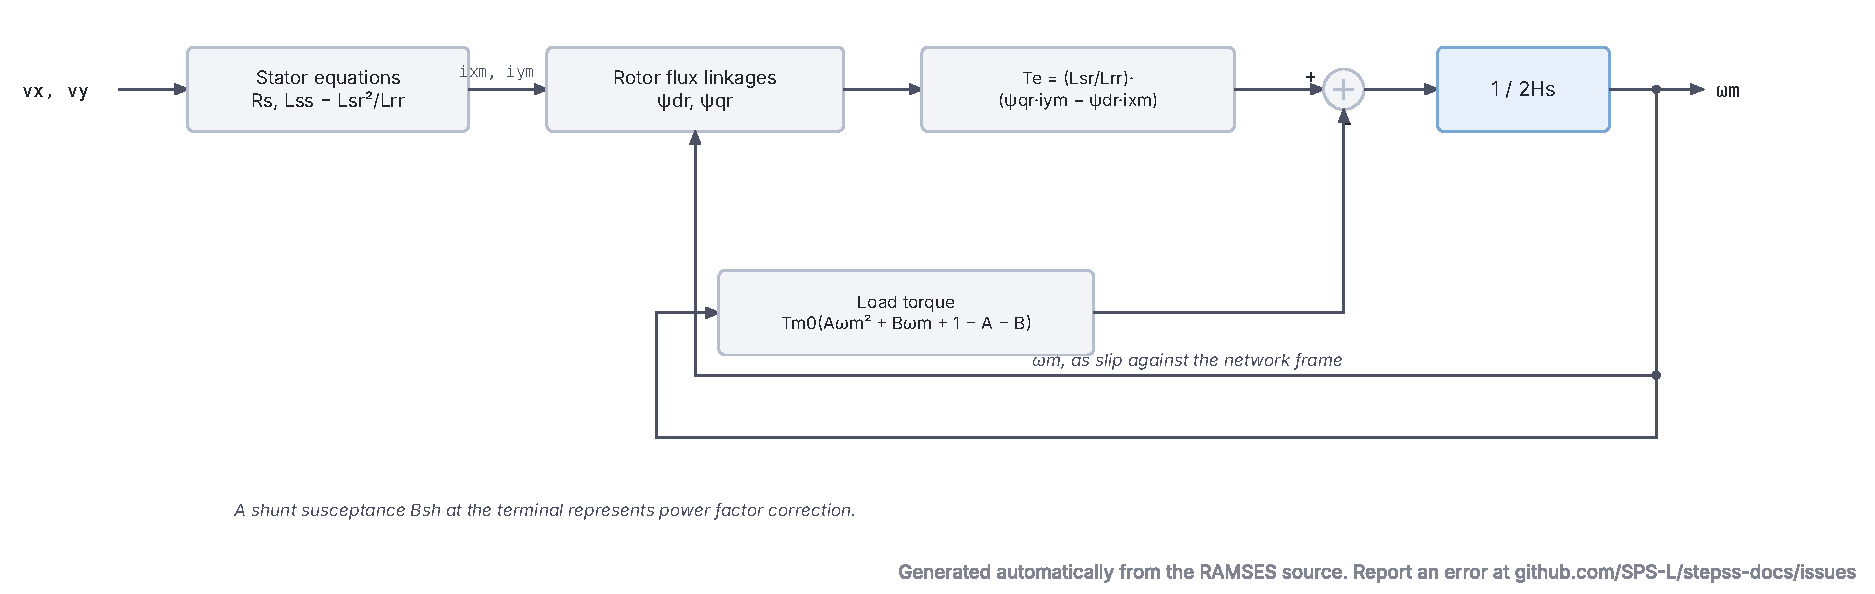
\includegraphics[width=0.98\linewidth]{figures/inj-indmach1-light}
\caption{Single-cage induction machine block diagram.}
\end{figure}

\subsection{Scientific Description}\label{model-inj-indmach:scientific-description}

The machine uses the standard \(d\)-\(q\) reference-frame formulation with \(L_{ss} = L_{sr} + L_{ls}\) and \(L_{rr} = L_{sr} + L_{lr}\). The rotor flux-linkage equations are:

\[\frac{d\psi_{dr}}{dt} = \omega_0\left(-\frac{R_r}{L_{rr}}\psi_{dr} + \frac{L_{sr} R_r}{L_{rr}} i_{ym} - (\omega - \omega_m)\psi_{qr}\right)\]

\[\frac{d\psi_{qr}}{dt} = \omega_0\left(-\frac{R_r}{L_{rr}}\psi_{qr} + \frac{L_{sr} R_r}{L_{rr}} i_{xm} + (\omega - \omega_m)\psi_{dr}\right)\]

where \(\omega_0 = 2\pi f_{\mathrm{nom}}\) and \(\omega_m\) is the rotor mechanical speed. The equations for the stator (with shunt susceptance \(B_{\mathrm{sh}}\)) are:

\[R_s i_{ym} + \left(L_{ss} - \frac{L_{sr}^2}{L_{rr}}\right)\omega\, i_{xm} + \frac{L_{sr}}{L_{rr}}\omega\,\psi_{qr} = v_y\]

\[R_s i_{xm} - \left(L_{ss} - \frac{L_{sr}^2}{L_{rr}}\right)\omega\, i_{ym} - \frac{L_{sr}}{L_{rr}}\omega\,\psi_{dr} = v_x\]

The rotor speed dynamics follow the swing equation:

\[\frac{d\omega_m}{dt} = \frac{T_e - T_m}{2H}\]

where the electromagnetic torque is:

\[T_e = \frac{L_{sr}}{L_{rr}}\left(-\psi_{dr} i_{xm} + \psi_{qr} i_{ym}\right)\]

and the mechanical torque is the quadratic load curve:

\[T_m = T_{m0}\left(A\,\omega_m^2 + B\,\omega_m + 1 - A - B\right)\]

\subsection{Parameters}\label{model-inj-indmach:parameters}

\begin{small}\begin{longtable}[]{@{}
  >{\raggedright\arraybackslash}p{(\linewidth - 8\tabcolsep) * \real{0.1166}}
  >{\raggedright\arraybackslash}p{(\linewidth - 8\tabcolsep) * \real{0.1716}}
  >{\raggedright\arraybackslash}p{(\linewidth - 8\tabcolsep) * \real{0.5691}}
  >{\raggedright\arraybackslash}p{(\linewidth - 8\tabcolsep) * \real{0.1428}}
@{}}
\toprule\noalign{}
\begin{minipage}[b]{\linewidth}\raggedright
\#
\end{minipage} & \begin{minipage}[b]{\linewidth}\raggedright
Name
\end{minipage} & \begin{minipage}[b]{\linewidth}\raggedright
Description
\end{minipage} & \begin{minipage}[b]{\linewidth}\raggedright
Unit
\end{minipage} \\
\midrule\noalign{}
\endhead
\bottomrule\noalign{}
\endlastfoot
1 & \texttt{SNOM} & Machine nominal apparent power (0 = infer from \texttt{LF}) & MVA \\
2 & \texttt{RS} & Stator resistance & pu \\
3 & \texttt{Lls} & Stator leakage inductance & pu \\
4 & \texttt{LSR} & Magnetizing inductance & pu \\
5 & \texttt{RR} & Rotor resistance & pu \\
6 & \texttt{Llr} & Rotor leakage inductance & pu \\
7 & \texttt{H} & Machine inertia constant & s \\
8 & \texttt{A} & Quadratic torque-speed coefficient & \\
9 & \texttt{B} & Linear torque-speed coefficient & \\
10 & \texttt{LF} & Load factor (for SNOM inference) & \\
\end{longtable}\end{small}

\subsection{State Variables}\label{model-inj-indmach:state-variables}

\begin{small}\begin{longtable}[]{@{}ll@{}}
\toprule\noalign{}
Variable & Description \\
\midrule\noalign{}
\endhead
\bottomrule\noalign{}
\endlastfoot
\texttt{iy} & \(y\)-component of stator current \\
\texttt{ix} & \(x\)-component of stator current \\
\texttt{psidr} & \(d\)-axis rotor flux linkage \\
\texttt{psiqr} & \(q\)-axis rotor flux linkage \\
\texttt{omegam} & Rotor mechanical speed \\
\end{longtable}\end{small}

\textbf{Observables:} \texttt{P}, \texttt{Qmot+comp}, \texttt{Qmot}, \texttt{omega}, \texttt{Tm}

\subsection{Usage Example}\label{model-inj-indmach:usage-example}

\begin{Verbatim}
INJEC  INDMACH1  MTR1  BUS_MV
      # FP FQ P Q: share of the power-flow injection (FP, FQ) or initial power (P in MW, Q in Mvar)
      1.  1.  0.  0.
      # SNOM: Machine nominal apparent power, 0 = infer from LF (MVA)
      10.0
      # RS: Stator resistance (pu (machine base))
      0.01
      # Lls: Stator leakage inductance (pu (machine base))
      0.10
      # LSR: Magnetizing inductance (pu (machine base))
      2.50
      # RR: Rotor resistance (pu (machine base))
      0.015
      # Llr: Rotor leakage inductance (pu (machine base))
      0.10
      # H: Inertia constant (s)
      1.5
      # A: Quadratic coefficient of load torque vs speed
      0.8
      # B: Linear coefficient of load torque vs speed
      0.1
      # LF: Load factor, initial P over SNOM, used only when SNOM = 0
      0.0
;
\end{Verbatim}

\begin{center}\rule{0.5\linewidth}{0.5pt}\end{center}

\section{\texorpdfstring{INDMACH2 (\texttt{inj\_indmach2}): Double-Cage Induction Machine}{INDMACH2 (inj\_indmach2): Double-Cage Induction Machine}}\label{model-inj-indmach:indmach2-inj_indmach2-double-cage-induction-machine}

\subsection{Description}\label{model-inj-indmach:description-1}

A double-cage (double-rotor-circuit) induction machine model following the Eurostag formulation. Two parallel rotor cages allow more accurate representation of the machine's impedance-vs-frequency characteristic, which is especially important for the starting transient. The model structure mirrors \texttt{inj\_indmach1} but includes a second set of rotor flux states.

\begin{figure}[htbp]
\centering
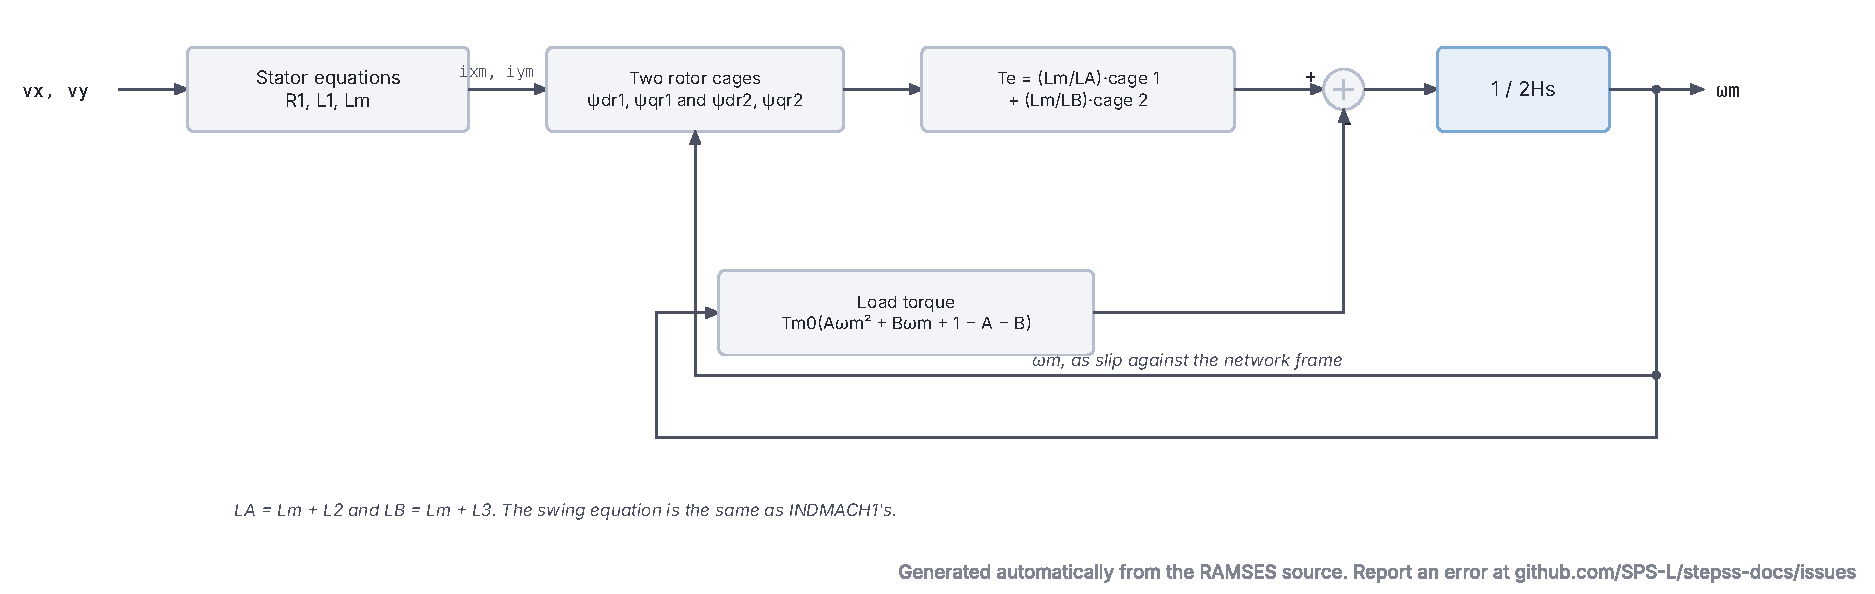
\includegraphics[width=0.98\linewidth]{figures/inj-indmach2-light}
\caption{Double-cage induction machine block diagram.}
\end{figure}

\subsection{Scientific Description}\label{model-inj-indmach:scientific-description-1}

The machine has parameters: stator resistance \(R_1\), stator leakage \(L_1\), magnetizing inductance \(L_m\), cage-1 resistance \(R_2\) and leakage \(L_2\), cage-2 resistance \(R_3\) and leakage \(L_3\). The state vector is \((\psi_{dr1},\psi_{qr1},\psi_{dr2},\psi_{qr2},\omega_m)\) with flux-linkage equations for each cage:

\[\frac{d\psi_{dr1}}{dt} = \omega_0\left(-\frac{R_2}{L_{A}}\psi_{dr1} + \frac{L_m R_2}{L_{A}} i_{ym} - (\omega - \omega_m)\psi_{qr1}\right)\]

\[\frac{d\psi_{dr2}}{dt} = \omega_0\left(-\frac{R_3}{L_{B}}\psi_{dr2} + \frac{L_m R_3}{L_{B}} i_{ym} - (\omega - \omega_m)\psi_{qr2}\right)\]

where \(L_A = L_m + L_2\) and \(L_B = L_m + L_3\). The total electromagnetic torque combines contributions from both cages:

\[T_e = \frac{L_m}{L_A}\left(-\psi_{dr1} i_{xm} + \psi_{qr1} i_{ym}\right) + \frac{L_m}{L_B}\left(-\psi_{dr2} i_{xm} + \psi_{qr2} i_{ym}\right)\]

The swing equation is identical to \texttt{inj\_indmach1}.

\subsection{Parameters}\label{model-inj-indmach:parameters-1}

\begin{small}\begin{longtable}[]{@{}llll@{}}
\toprule\noalign{}
\# & Name & Description & Unit \\
\midrule\noalign{}
\endhead
\bottomrule\noalign{}
\endlastfoot
1 & \texttt{SNOM} & Machine MVA rating (0 = infer from \texttt{LF}) & MVA \\
2 & \texttt{R1} & Stator resistance & pu \\
3 & \texttt{L1} & Stator leakage inductance & pu \\
4 & \texttt{Lm} & Magnetizing inductance & pu \\
5 & \texttt{R2} & First cage resistance & pu \\
6 & \texttt{L2} & First cage leakage inductance & pu \\
7 & \texttt{R3} & Second cage resistance & pu \\
8 & \texttt{L3} & Second cage leakage inductance & pu \\
9 & \texttt{H} & Inertia constant & s \\
10 & \texttt{A} & Quadratic torque-speed coefficient & \\
11 & \texttt{B} & Linear torque-speed coefficient & \\
12 & \texttt{LF} & Load factor (for SNOM inference) & \\
\end{longtable}\end{small}

\subsection{State Variables}\label{model-inj-indmach:state-variables-1}

\begin{small}\begin{longtable}[]{@{}ll@{}}
\toprule\noalign{}
Variable & Description \\
\midrule\noalign{}
\endhead
\bottomrule\noalign{}
\endlastfoot
\texttt{iy} & \(y\)-component of stator current \\
\texttt{ix} & \(x\)-component of stator current \\
\texttt{psidr1} & \(d\)-axis flux of first rotor cage \\
\texttt{psiqr1} & \(q\)-axis flux of first rotor cage \\
\texttt{psidr2} & \(d\)-axis flux of second rotor cage \\
\texttt{psiqr2} & \(q\)-axis flux of second rotor cage \\
\texttt{omegam} & Rotor mechanical speed \\
\end{longtable}\end{small}

\textbf{Observables:} \texttt{P}, \texttt{Qmot+comp}, \texttt{Qmot}, \texttt{omega}

\subsection{Usage Example}\label{model-inj-indmach:usage-example-1}

\begin{Verbatim}
INJEC  INDMACH2  MTR2  BUS_MV
      # FP FQ P Q: share of the power-flow injection (FP, FQ) or initial power (P in MW, Q in Mvar)
      1.  1.  0.  0.
      # SNOM: Machine nominal apparent power, 0 = infer from LF (MVA)
      10.0
      # R1: Stator resistance (pu (machine base))
      0.01
      # L1: Stator leakage inductance (pu (machine base))
      0.08
      # Lm: Magnetizing inductance (pu (machine base))
      2.00
      # R2: First cage resistance (pu (machine base))
      0.02
      # L2: First cage leakage inductance (pu (machine base))
      0.06
      # R3: Second cage resistance (pu (machine base))
      0.04
      # L3: Second cage leakage inductance (pu (machine base))
      0.10
      # H: Inertia constant (s)
      1.5
      # A: Quadratic coefficient of load torque vs speed
      0.8
      # B: Linear coefficient of load torque vs speed
      0.1
      # LF: Load factor, initial P over SNOM, used only when SNOM = 0
      0.0
;
\end{Verbatim}

\begin{center}\rule{0.5\linewidth}{0.5pt}\end{center}

\section{\texorpdfstring{INDM1 (\texttt{inj\_INDM1}): Alternative Induction Machine}{INDM1 (inj\_INDM1): Alternative Induction Machine}}\label{model-inj-indmach:indm1-inj_indm1-alternative-induction-machine}

The data-file model name is \texttt{INDM1} (or \texttt{inj\_INDM1}).

\begin{docsnote}{Note}

Callable since 3.79. Earlier releases compiled this model under no name, so a data file referring to it was rejected. For built-in single-cage motors, use \texttt{INDMACH1} instead.

\end{docsnote}

\subsection{Description}\label{model-inj-indmach:description-2}

An alternative single-cage induction machine model that uses the \texttt{INI\_indmach1} helper function for initialization. It is equivalent in physics to \texttt{inj\_indmach1} but implements the equations using RAMSES \texttt{.txt}-style model syntax with explicit state initialization calls. This can simplify parameterization when the helper function's output is directly used.

\subsection{Scientific Description}\label{model-inj-indmach:scientific-description-2}

The model equations match those of \hyperref[model-inj-indmach:indmach1-inj_indmach1-single-cage-induction-machine]{\texttt{inj\_indmach1}}, whose block diagram applies here unchanged. The key distinction is the use of the \texttt{INI\_indmach1} function at parameter-evaluation time to pre-compute \(B_{\mathrm{sh}}\), \(T_{m0}\), and the initial flux linkages and rotor speed, rather than solving the initialization system in Fortran. With \(L_{ss} = L_{sr} + L_{ls}\) and \(L_{rr} = L_{sr} + L_{lr}\), the rotor flux equations are:

\[\frac{d\psi_{dr}}{dt} = 2\pi f_0 \left[ -\frac{R_R}{L_{rr}}\psi_{dr} + \frac{L_{SR} R_R}{L_{rr}} i_{ym} - (\omega - \omega_m)\psi_{qr} \right]\]

\[\frac{d\psi_{qr}}{dt} = 2\pi f_0 \left[ -\frac{R_R}{L_{rr}}\psi_{qr} + \frac{L_{SR} R_R}{L_{rr}} i_{xm} + (\omega - \omega_m)\psi_{dr} \right]\]

The rotor speed integral uses:

\[\frac{d\omega_m}{dt} = \frac{1}{2H}\left[\frac{L_{SR}}{L_{rr}}(-\psi_{dr} i_{xm} + \psi_{qr} i_{ym}) - T_{m0}(A\omega_m^2 + B\omega_m + 1 - A - B)\right]\]

with a lower limit of \(\omega_m \ge 0\).

\subsection{Parameters}\label{model-inj-indmach:parameters-2}

\begin{small}\begin{longtable}[]{@{}llll@{}}
\toprule\noalign{}
\# & Name & Description & Unit \\
\midrule\noalign{}
\endhead
\bottomrule\noalign{}
\endlastfoot
1 & \texttt{SNOM} & Machine MVA rating & MVA \\
2 & \texttt{RS} & Stator resistance & pu \\
3 & \texttt{Lls} & Stator leakage inductance & pu \\
4 & \texttt{LSR} & Magnetizing inductance & pu \\
5 & \texttt{RR} & Rotor resistance & pu \\
6 & \texttt{Llr} & Rotor leakage inductance & pu \\
7 & \texttt{H} & Inertia constant & s \\
8 & \texttt{A} & Quadratic torque-speed coefficient & \\
9 & \texttt{B} & Linear torque-speed coefficient & \\
10 & \texttt{LF} & Load factor & \\
\end{longtable}\end{small}

Computed internally: \texttt{BSH} (shunt susceptance), \texttt{TM0} (initial mechanical torque), \texttt{LSS}, \texttt{LRR}.

\subsection{State Variables}\label{model-inj-indmach:state-variables-2}

\begin{small}\begin{longtable}[]{@{}ll@{}}
\toprule\noalign{}
Variable & Description \\
\midrule\noalign{}
\endhead
\bottomrule\noalign{}
\endlastfoot
\texttt{Psidr} & \(d\)-axis rotor flux linkage \\
\texttt{Psiqr} & \(q\)-axis rotor flux linkage \\
\texttt{omegam} & Rotor mechanical speed \\
\texttt{iym}, \texttt{ixm} & Stator current components (on machine base) \\
\texttt{dPsidr}, \texttt{dPsiqr}, \texttt{domegam} & Time-derivative auxiliary states \\
\end{longtable}\end{small}

\textbf{Observables:} \texttt{omegam}

\subsection{Usage Example}\label{model-inj-indmach:usage-example-2}

\begin{Verbatim}
INJEC  INDM1  MTR3  BUS_MV
      # FP FQ P Q: share of the power-flow injection (FP, FQ) or initial power (P in MW, Q in Mvar)
      1.  1.  0.  0.
      # SNOM: Machine MVA rating (MVA)
      10.0
      # RS: Stator resistance (pu)
      0.01
      # Lls: Stator leakage inductance (pu)
      0.10
      # LSR: Magnetizing inductance (pu)
      2.50
      # RR: Rotor resistance (pu)
      0.015
      # Llr: Rotor leakage inductance (pu)
      0.10
      # H: Inertia constant (s)
      1.5
      # A: Quadratic torque-speed coefficient
      0.8
      # B: Linear torque-speed coefficient
      0.1
      # LF: Load factor
      0.0
;
\end{Verbatim}
